\section{NaFSI/TFSI solutions in ether solvents}

Among studied electrolytes for batteries are systems based on glymes. There were several works that considered diglyme~\cite{peo-diglyme-1,peo-diglyme-2,peo-diglyme-3} or other short glymes~\cite{na-dft-12,na-dft-14,na-interactions-1,na-dft-16,spectroscopy-structure-1,peo-na-glyme-1,peo-na-glyme-2,peo-na-glyme-3} as a solvent. Other systems are based on polymers, mostly poly(ethylene oxide) (PEO)~\cite{el-peo-2,ir-interactions-9,peo-na-tfsi-peo-1}. As sodium salts in such electrolytes NaFSI or NaTFSI were used~\cite{na-dft-12,na-dft-14,na-dft-16,peo-na-glyme-1,el-peo-2,ir-interactions-9,peo-na-tfsi-peo-1}. However, published MD results had different applied methodology and typically focused on only one of these anions and either on short oligoglyme molecules or on polymer chains. Thus, the study described in this section was an attempt to compare results for both anions and for three solvents with different lengths of the ether chain: monoglyme, tetraglyme, and PEO. This study was published in the article~\cite{peo-na}.

\subsection{System details}

Electrolytes considered in this work were NaFSI or NaTFSI solutions in monoglyme, tetraglyme or short PEO chains with 100~oxygen atoms each. Systems were constructed in such a way that the total number of ether oxygens was equal 600. Thus, the number of solvent molecules was 300, 120 and 6~for monoglyme, tetraglyme and PEO respectively. For each salt, two concentrations with 30 or 100 ion pairs were simulated, leading to Na/O ratios 1:20 or 1:6. These were the ratios studied experimentally~\cite{ir-interactions-9}. Initial structures for systems with PEO were prepared using Scigress~\cite{scigress}.

In this work, all systems were studied by classical MD. A timestep of 1.0~fs was used. Each of the systems was equilibrated in NpT ensemble with pressure 1~atm and temperature 303~K for 50~ns (glymes) or 100~ns (PEO). Then, 150-250~ns of trajectories in the NVT ensemble, with volume reproducing the equilibrated density in NpT ensemble, were recorded. Results for a~given system were averaged over 10~independent MD trajectories.

\subsection{Results}

RDFs for Na-O pairs for 1:6 electrolytes are presented in Figure~\ref{fig:peo-na-rdf-na-o}. The position of the maximum for Na-O$_{\text{E}}$ pair in every case is equal 2.36-2.37~{\AA} and does not depend on the anion, solvent molecule or salt concentration. In systems with FSI$^{-}$ anion it has a larger height than in systems with TFSI$^{-}$. For Na-O$_A$ pairs, the position of the maximum depends on the anion, for FSI$^{-}$ is located at the same distance as for Na-O$_E$, while for TFSI$^{-}$ it is at smaller distance - 2.3~{\AA}. Heights of the maxima are significantly smaller for FSI$^{-}$ anion than for TFSI$^{-}$. This difference suggests that Na$^{+}$ complexation by the FSI$^{-}$ anions is weaker.

The effect of weaker complexation by FSI$^{-}$ anion is seen in the integrated RDFs in Figure~\ref{fig:peo-na-rdf-int-na-o}. For 1:20 systems coordination by this anion is marginal, it is non-negligible only in the system with PEO, but is still less than 1~oxygen atom per cation. For all systems, it is visible that coordination by ether oxygen is preferred over coordination by the anion; however, this effect is weaker in concentrated solutions. Only in 1:6 NaTFSI-PEO system coordination to the anion is preferred over ether oxygen atoms (average number of oxygen atoms at distance 3.5~{\AA} equals 2.79 vs 2.64 for TFSI$^{-}$ and PEO respectively).

\begin{figure}[H]
    \centering
    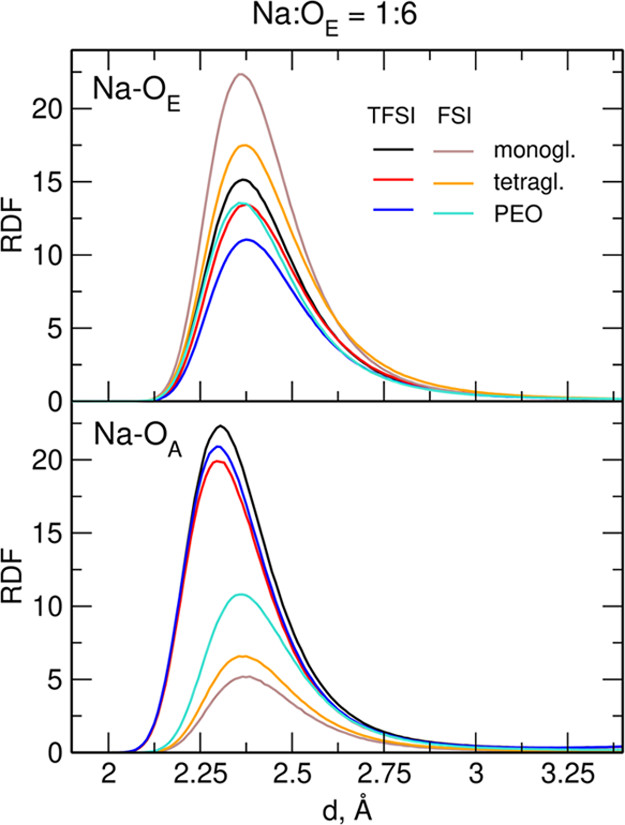
\includegraphics[width=0.4\textwidth]{img/3-structural-data-from-md-simulations/5-peo-na/rdf-na-o-1-6.png}
    \singlespacing
    \caption{Radial distribution functions for Na-O atom pairs in 1:6 electrolytes (O$_{\text{E}}$ - ether oxygen atom, O$_{\text{A}}$ - oxygen atom from anion)}
    \label{fig:peo-na-rdf-na-o}
\end{figure}

\begin{figure}[H]
    \centering
    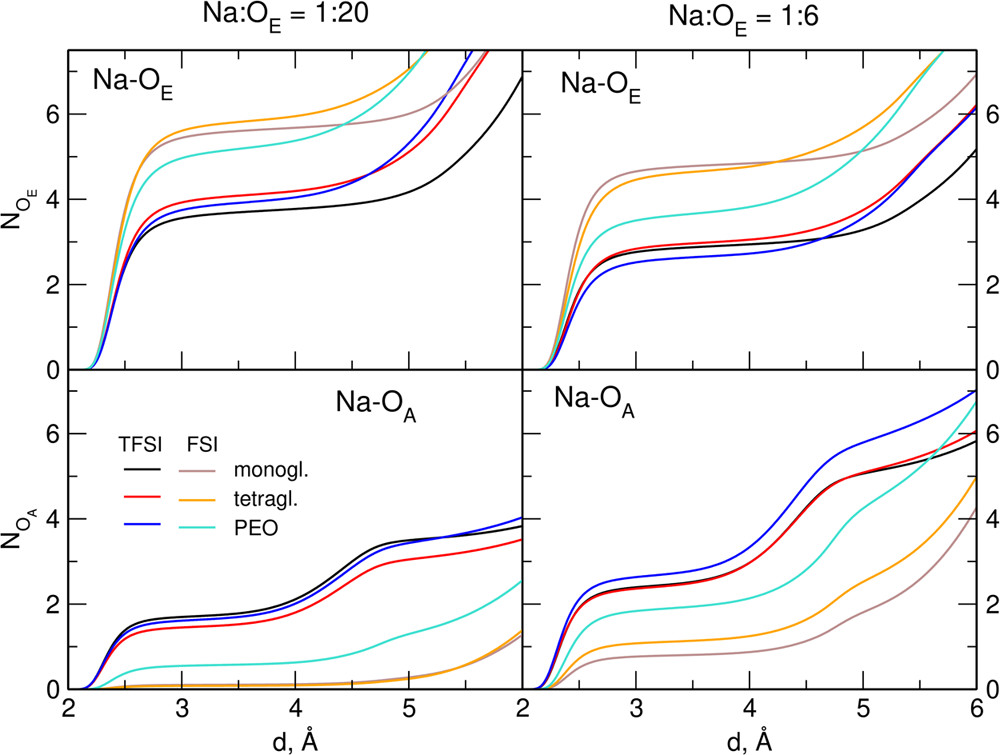
\includegraphics[width=0.6\textwidth]{img/3-structural-data-from-md-simulations/5-peo-na/rdf-int-na-o.png}
    \singlespacing
    \caption{Integrated Na-O RDFs for 1:20 and 1:6 systems}
    \label{fig:peo-na-rdf-int-na-o}
\end{figure}

To gain a better understanding of the cation-solvent or cation-anion aggregates, histograms of coordination numbers (CNs) were plotted. Selected representative examples are shown in Figure~\ref{fig:peo-na-histograms-chosen}. In the 1:20 NaFSI electrolyte in tetraglyme the most probable number of ether oxygen atoms coordinating the cation is~6. At bigger concentrations, this distribution becomes wider and for PEO all values between 2~and~6 have similar probability. For NaTFSI systems, all distributions are broad and abundance of CNs = 3, 4 or~6 is comparable. Figure~\ref{fig:peo-na-histograms-chosen}(b) shows anion CNs distribution for 1:20 systems in monoglyme, here the effect of more frequent coordination by TFSI$^{-}$ anions compared to FSI$^{-}$ anions, as it was seen in the RDFs, is also present. For TFSI$^{-}$ the most probable CNs are~2 and next 0~and~4 while for FSI$^{-}$ the most probable value for more than 90\% of cations is~0. Finallly, Figure~\ref{fig:peo-na-histograms-chosen}c shows the distribution of number of cations coordinated to PEO molecule in 1:6 system. Here, the maximum for the distribution for NaFSI electrolyte is at about 20~cations whereas for NaTFSI at about 15~cations.

\begin{figure}[H]
    \centering
    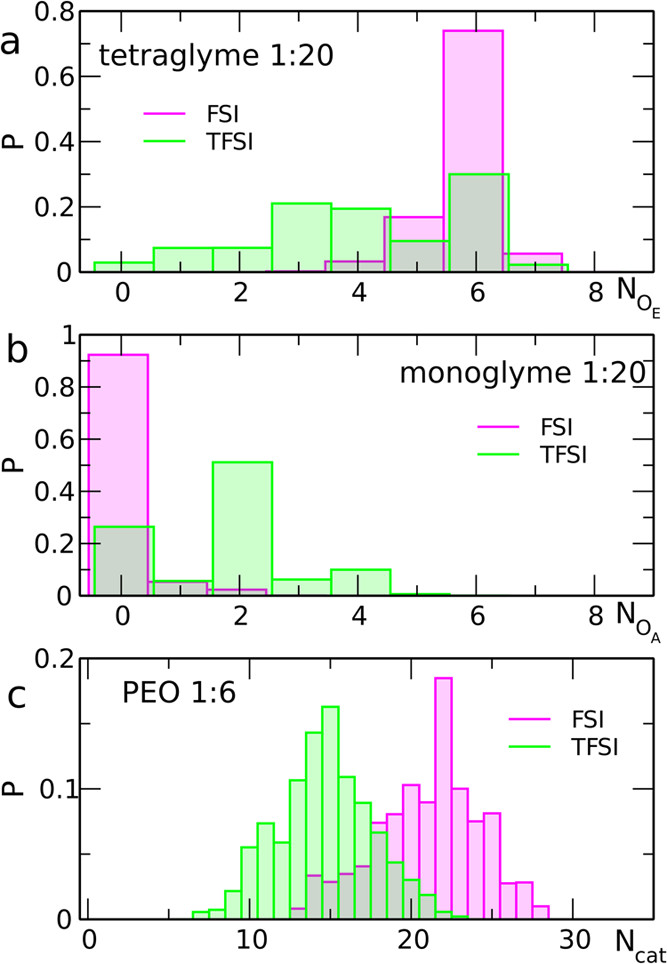
\includegraphics[width=0.4\textwidth]{img/3-structural-data-from-md-simulations/5-peo-na/histograms-chosen.png}
    \caption{Distribution of the number of ether oxygen atoms coordinated to Na$^{+}$ (a), of the number of anion oxygen atoms coordinated to Na$^{+}$ (b), and of the number of Na$^{+}$ ions coordinated to PEO molecules (c)}
    \label{fig:peo-na-histograms-chosen}
\end{figure}

\begin{figure}[ht]
    \centering
    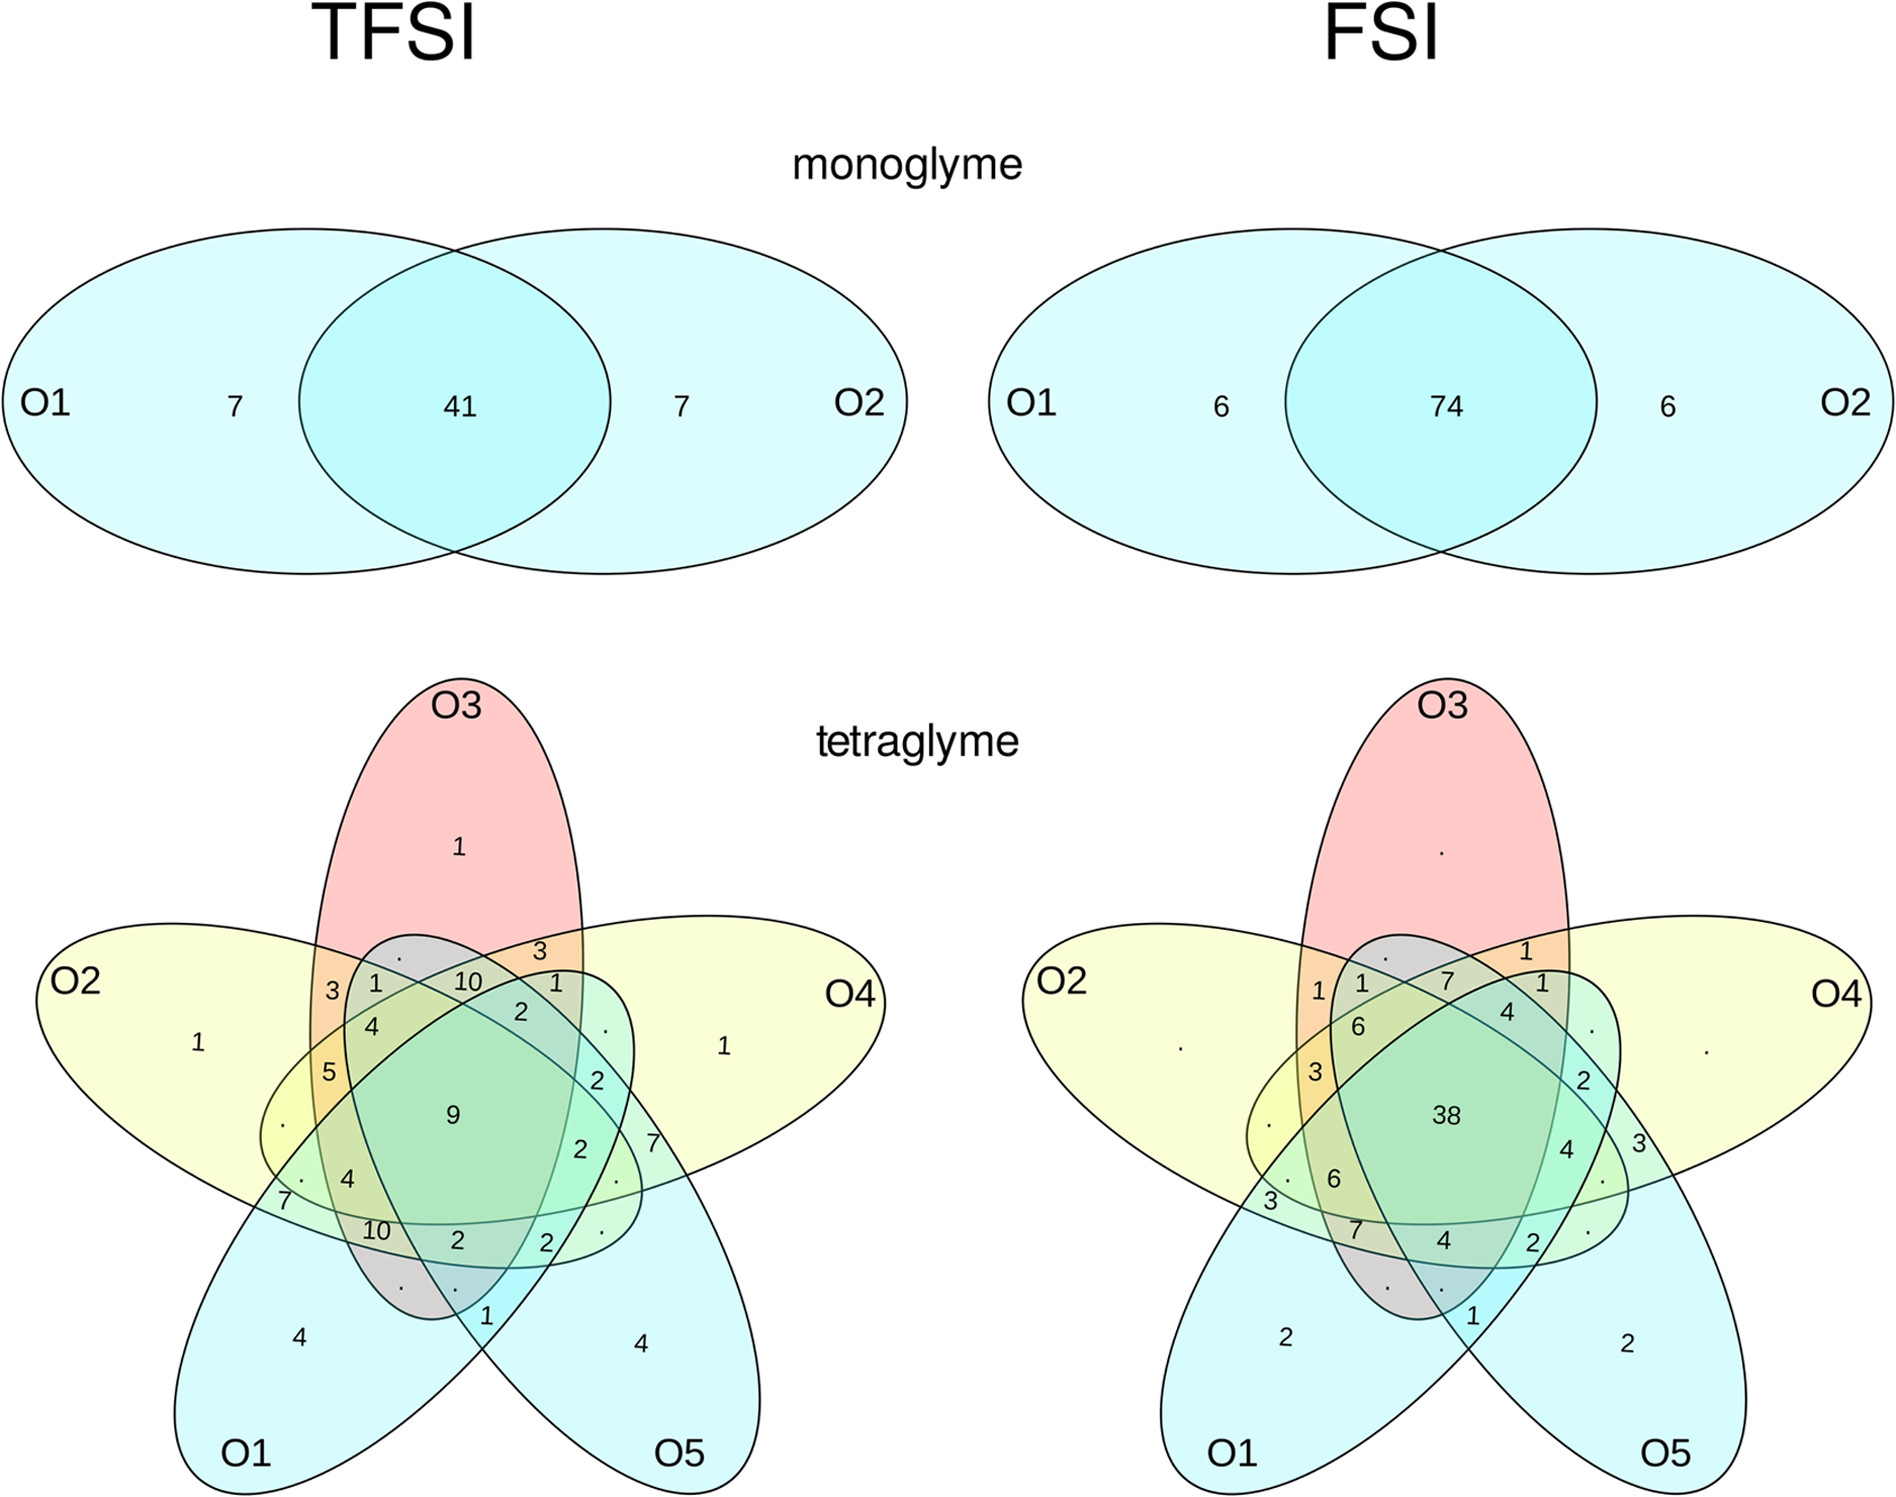
\includegraphics[width=0.6\textwidth]{img/3-structural-data-from-md-simulations/5-peo-na/venn.png}
    \singlespacing
    \caption{Venn diagrams showing the connectivity between Na$^{+}$ ion and oxygen atoms of the monoglyme and tetraglyme molecules in 1:6 electrolytes, values lower than 1\% are displayed as dots}
    \label{fig:peo-na-venn}
\end{figure}

For the analysis of binding pattern in mono- and tetraglyme systems, Venn diagrams were prepared showing the percentage of solvent molecules engaging specified subset of oxygen atoms in interactions with sodium cations, the graphs were symmetrized with respect to equivalent atoms. For example, for plot for monoglyme-NaFSI connections shows that 74\% of monoglyme molecules interact with Na$^{+}$ cations with both oxygen atoms, and 12\% with one of them, this percentage is divided equally to the two indistinguishable O~atoms. Such diagrams for 1:6 systems are presented in Figure~\ref{fig:peo-na-venn}. For monoglyme in NaFSI the percentage of molecules that interact through both oxygen atoms is almost two times larger than in the NaTFSI electrolyte. In addition, in tetraglyme this ratio is about 4:1 (38\% and 9\% respectively). For the NaTFSI system in tetraglyme it is more probable that 3~consecutive O~atoms are interacting with Na$^{+}$ (20\%) while in NaFSI it is less abundant configuration (14\%). In more than 80\% cases, if more than one atom from tetraglyme interacts with sodium cations, the interacting atoms are consecutive oxygen atoms.

\begin{figure}[H]
    \centering
    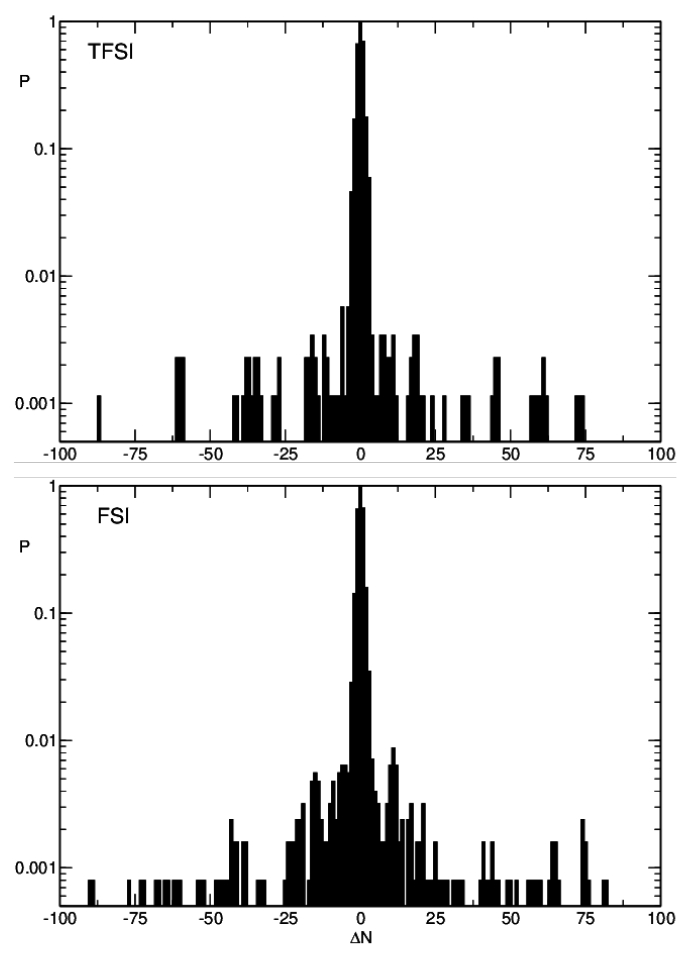
\includegraphics[width=0.4\textwidth]{img/3-structural-data-from-md-simulations/5-peo-na/peo-dn.png}
    \singlespacing
    \caption{Distribution of the probability that an oxygen atom positioned at the site $\Delta N$ is coordinated to the Na$^{+}$ cation, interacting with the oxygen atom at the site N = 0 in the 1:6 PEO-based electrolytes}
    \label{fig:peo-na-peo-dn}
\end{figure}

For PEO it was impossible to visualize the binding pattern using Venn diagrams, so in Figure~\ref{fig:peo-na-peo-dn} the probability is plotted that the same cation that interacts with the oxygen atom at position $N = 0$, simultaneously interacts with atom positioned $\Delta N$ sites apart. Significant probability is obtained only for $| \Delta N |$ not larger than~3, but it is worth noting that there are several values with non-zero probability corresponding to $| \Delta N |$ larger than~20. These are the cases where a~loop of PEO chain occurs and enables Na$^{+}$ coordination to its distant parts.

\begin{figure}[ht]
    \centering
    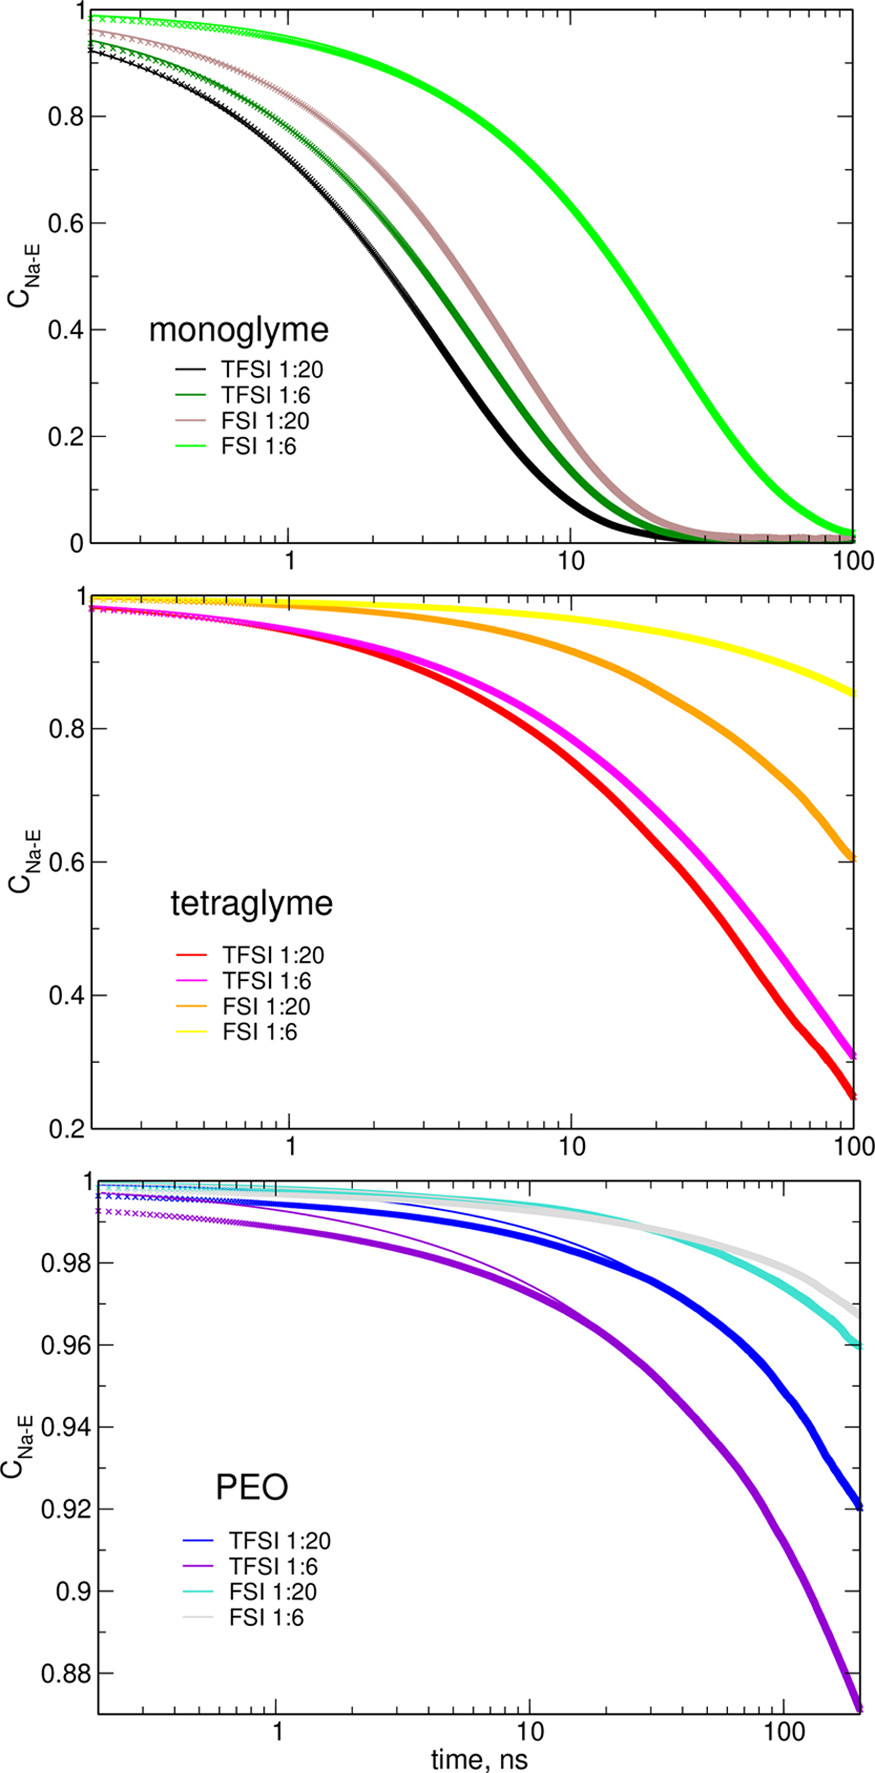
\includegraphics[width=0.4\textwidth]{img/3-structural-data-from-md-simulations/5-peo-na/residence.png}
    \caption{Residence time autocorrelation function for Na-ether interactions. Lines are fits to the data}
    \label{fig:peo-na-residence}
\end{figure}

As for the previously described systems, the residence time autocorrelation functions were calculated and are presented in Figure~\ref{fig:peo-na-residence}. Residence times for ether molecules $\tau_{\text{E}}$ were calculated by fitting stretched exponential function $e^{-\left( \frac{t}{\tau_{\text{E}}} \right)^{\alpha}}$ to the obtained data. $\tau_{\text{E}}$ values are shown in Table~\ref{tab:peo-na-residence}. Due to larger viscosities of tetraglyme and PEO based systems, during the simulation time, only for monoglymes the autocorrelation functions reached~0. For all systems, residence times in NaFSI electrolytes are larger than in NaTFSI solutions. This suggests that NaFSI salt promotes more stable Na$^{+}$ binding to solvent molecules and thus slower exchange of ions in the solvation shell. For PEO-based electrolytes in NaFSI solutions residence times increase in 1:6 electrolyte compared to 1:20 one, while for NaTFSI the effect is opposite. A~possible explanation is the different mechanism of ion transport due to larger number of cation-anion interactions in NaTFSI solutions which increases the probability of Na$^{+}$ exchange between anions.

\begin{table}[ht]
  \centering
  \caption{Residence times $\tau_{\text{E}}$ for ether molecules in nanoseconds}
  \label{tab:peo-na-residence}
\begin{tabular}{cc}
\toprule
system                              & $\tau_{\text{E}}$, ns                    \\
\midrule
NaTFSI – monoglyme 1:20             & 3.5                       \\
NaTFSI – monoglyme 1:6              & 4.7                       \\
NaFSI – monoglyme 1:20              & 6.1                       \\
NaFSI – monoglyme 1:6               & 23                        \\
NaTFSI – tetraglyme 1:20            & 61                        \\
NaTFSI – tetraglyme 1:6             & 79                        \\
NaFSI – tetraglyme 1:20             & 250                       \\
NaFSI – tetraglyme 1:6              & 1710                      \\
NaTFSI – PEO 1:20                   & 9090                      \\
NaTFSI – PEO 1:6                    & 7020                      \\
NaFSI – PEO 1:20                    & 27500                     \\
NaFSI – PEO 1:6 & 98100 \\
\bottomrule
\end{tabular}
\end{table}

\begin{figure}[ht]
    \centering
    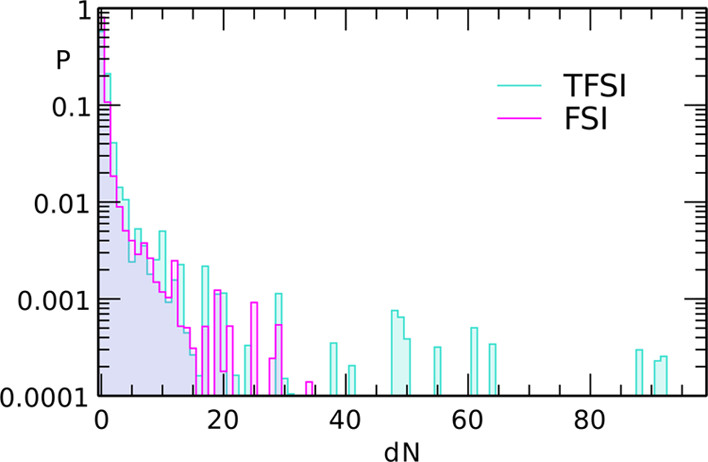
\includegraphics[width=0.4\textwidth]{img/3-structural-data-from-md-simulations/5-peo-na/peo-dn-2.png}
    \caption{Probability of the displacement of Na$^{+}$ iond by $dN$ sites along the PEO chain in 1:6 Na(T)FSI/PEO electrolytes after 250~ns of simulations}
    \label{fig:peo-na-peo-dn-2}
\end{figure}

For the PEO-based electrolytes in addition to data about distances between coordinating oxygen atoms, the dynamics of ions movement along the chains is also interesting. Figure~\ref{fig:peo-na-peo-dn-2} presents the probability that sodium cation moved after 250~ns of simulation by $dN$ from its original position. For the majority of cations displacements are small and do not exceed five binding sites. For $dN$ values between 5~and 15~probabilities are below 1\%. These changes of binding sites could be related to cation movements along the PEO chain. There are also less probable cases of large $dN$ values, up to tens of sites. They may be related to breaking PEO-cation interaction at one site and association of the cation to another binding atom, which due to spatial loop of the PEO chain may be a~distant one (in values of $dN$). These changes are more probable in the electrolyte with TFSI$^{-}$ anion.

Presented results showed differences in coordination numbers and binding patterns of ether molecules between systems with FSI$^{-}$ and TFSI$^{-}$ anions; the latter interact more frequently with sodium cations, while the former favor sodium-ether binding.

The total number of coordinating oxygen atoms decreases with increasing salt concentration. This effect stands in agreement with coordination numbers derived from experimental Raman spectra for NaTFSI solutions in carbonate solvents~\cite{peo-na-experimental-raman-1} or mixed molecular/IL electrolytes~\cite{peo-na-experimental-raman-2}. Observed for monoglyme trend of increasing probability of cation-anion coordination for increasing salt concentration is in agreement with results for polarizable MD simulations for NaTFSI solutions~\cite{peo-na-glyme-3}. However, this trend observed from MD simulations for PEO differs from conclusions made from experimental Raman spectra~\cite{ir-interactions-9}, where at low salt load almost all TFSI$^{-}$ anions are "free" while only about 2/3 of FSI$^{-}$ anions do not interact with sodium cation. On the other side, the experimental data for diluted solutions in tetra- or pentaglyme~\cite{na-dft-12} stands in an agreement with trends obtained from MD simulations. The mentioned discrepancy for PEO with simultaneous compatibility between MD and experimental results, suggest that interactions in PEO have a~different character that for short glymes and would need a~specifically developed FF to be correctly described in MD simulation.

\cleardoublepage